\documentclass[border=4pt,12pt]{standalone}
% House style for redrawn exam diagrams (diagram-v4: 0.4pt lines, filled -latex arrows, fine dashes; stipple and hatching drawn as real dots/lines (no PDF/SVG patterns, so they render in every browser and at any scale); transparent background). Every figure \input's this.
\usepackage{amsmath,amssymb}
\usepackage{txfonts}
\usepackage{pdfrender,xcolor}
% \halo{text}: label on shading. The shading stops just around each letter's outline (a thin knock-out that follows the
% glyphs, like the papers' typesetting), never a box. Owner: "I don't want a box around the text".
\newcommand{\halo}[1]{\leavevmode\rlap{\pdfrender{TextRenderingMode=2,LineWidth=2.2pt,LineJoinStyle=1,StrokeColor=white,FillColor=white}#1}#1}
\usepackage{tikz,pgfplots}
\pgfplotsset{compat=1.18}
\usetikzlibrary{arrows.meta,calc,angles,quotes,patterns,patterns.meta,intersections,positioning,decorations.markings,shapes.geometric}
% Stipple and hatching are drawn as actual dots / lines clipped to the region (path picture), NOT as pattern fills:
% SVG <pattern> fills vanish or blur when browsers scale the image, so the owner could not see the shading.
% Each dot is a 0.72pt square (keeps SVGs small; reads as a dot at print size). Dots sit on one global staggered grid, so neighbouring regions line up.
\makeatletter
\newdimen\ex@x \newdimen\ex@y \newdimen\ex@xa \newdimen\ex@ya \newdimen\ex@xb \newdimen\ex@yb \newcount\ex@row
\def\exam@stipplecolor{black!75}\def\exam@dotr{0.42pt}\def\exam@dotgap{2.5}
\def\ex@rowdots{\ifdim\ex@x<\ex@xb \pgfpathrectangle{\pgfqpoint{\dimexpr\ex@x-0.36pt\relax}{\dimexpr\ex@y-0.36pt\relax}}{\pgfqpoint{0.72pt}{0.72pt}}\advance\ex@x by \exam@dotgap pt\relax\expandafter\ex@rowdots\fi}
\def\exam@stipple{%
  \pgftransformreset% dots are sized in real points even inside scaled pictures
  \pgfpointanchor{path picture bounding box}{south west}\ex@xa=\pgf@x \ex@ya=\pgf@y
  \pgfpointanchor{path picture bounding box}{north east}\ex@xb=\pgf@x \ex@yb=\pgf@y
  \pgfsetfillcolor{\exam@stipplecolor}\pgfmathsetmacro\ex@h{\exam@dotgap/2}%
  \pgfmathtruncatemacro\ex@r{floor(\ex@ya/\ex@h)-1}\ex@row=\ex@r\relax
  \ex@y=\ex@r\dimexpr\ex@h pt\relax
  \loop\ifdim\ex@y<\ex@yb
    \pgfmathtruncatemacro\ex@c{floor(\ex@xa/\exam@dotgap)-1}\ex@x=\ex@c\dimexpr\exam@dotgap pt\relax
    \ifodd\ex@row \advance\ex@x by \ex@h pt\fi
    \ex@rowdots
    \advance\ex@y by \ex@h pt \advance\ex@row by 1
    \ifnum\numexpr\ex@row-(\ex@row/4)*4\relax=0 \pgfusepath{fill}\fi% flush every 4 rows: bounded TeX memory, few clip copies in the SVG
  \repeat\pgfusepath{fill}}
\newdimen\ex@d
\def\exam@hatch#1{% #1 = 1 for /, -1 for \ ; lines 45 degrees, 3pt apart
  \pgftransformreset
  \pgfpointanchor{path picture bounding box}{south west}\ex@xa=\pgf@x \ex@ya=\pgf@y
  \pgfpointanchor{path picture bounding box}{north east}\ex@xb=\pgf@x \ex@yb=\pgf@y
  \ex@d=\dimexpr\ex@yb-\ex@ya\relax \ex@x=\dimexpr\ex@xa-\ex@d\relax
  \loop\ifdim\ex@x<\ex@xb
    \ifnum#1>0 \pgfpathmoveto{\pgfqpoint{\ex@x}{\ex@ya}}\pgfpathlineto{\pgfqpoint{\dimexpr\ex@x+\ex@d\relax}{\ex@yb}}%
    \else \pgfpathmoveto{\pgfqpoint{\ex@x}{\ex@yb}}\pgfpathlineto{\pgfqpoint{\dimexpr\ex@x+\ex@d\relax}{\ex@ya}}\fi
    \advance\ex@x by 4.24pt
  \repeat
  \pgfsetlinewidth{0.4pt}\pgfsetstrokecolor{black}\pgfusepath{stroke}}
\def\examstipple{\exam@stipple}\def\examhatch{\exam@hatch}\def\examsetstipplecolor#1{\def\exam@stipplecolor{#1}}\def\examsetdotgap#1{\def\exam@dotgap{#1}}
\makeatother
% (legacy pattern kept for old files)
% staggered stipple like the NESA papers' dotted shading
\pgfdeclarepatternformonly{exam stipple}{\pgfpointorigin}{\pgfqpoint{2.2pt}{2.2pt}}{\pgfqpoint{2.2pt}{2.2pt}}{%
  \pgfpathcircle{\pgfqpoint{0.55pt}{0.55pt}}{0.42pt}\pgfpathcircle{\pgfqpoint{1.65pt}{1.65pt}}{0.42pt}\pgfusepath{fill}}
\tikzset{
  every picture/.style={line width=0.6pt, >={Latex[length=2mm,width=1.3mm]}},
  curve/.style={line width=0.6pt},
  open arrow/.style={-{Latex[length=2mm,width=1.3mm]}},  % owner: filled -latex heads everywhere, no open chevrons
  aux/.style={dash pattern=on 2pt off 1.5pt, line width=0.6pt},
  shade/.code={\def\exA{#1}\def\exB{none}\ifx\exA\exB\else\pgfkeysalso{fill=black!18}\fi},
  shade/.default=on,
  shade dots/.style={fill=none, path picture={\examstipple}},
  stipple color/.code={\examsetstipplecolor{#1}},
  stipple gap/.code={\examsetdotgap{#1}},
  shade dense dots/.style={fill=none, stipple gap=1.6, path picture={\examstipple}},
  shade hatch/.style={fill=none, path picture={\examhatch{1}}},
  shade hatch reverse/.style={fill=none, path picture={\examhatch{-1}}},
  shade solid/.style={fill=black},
  pt/.style={circle, fill, inner sep=1.1pt},
  open pt/.style={circle, draw, fill=white, inner sep=1.1pt},
}
\pgfplotsset{
  exam axes/.style={axis lines=middle, axis line style={->}, xlabel={$x$}, ylabel={$y$},
    xlabel style={anchor=west}, ylabel style={anchor=south}, tick label style={font=\small},
    every axis plot/.append style={line width=0.6pt, black}, samples=200, clip=false,
    enlargelimits=false, axis on top},
}

\begin{document}
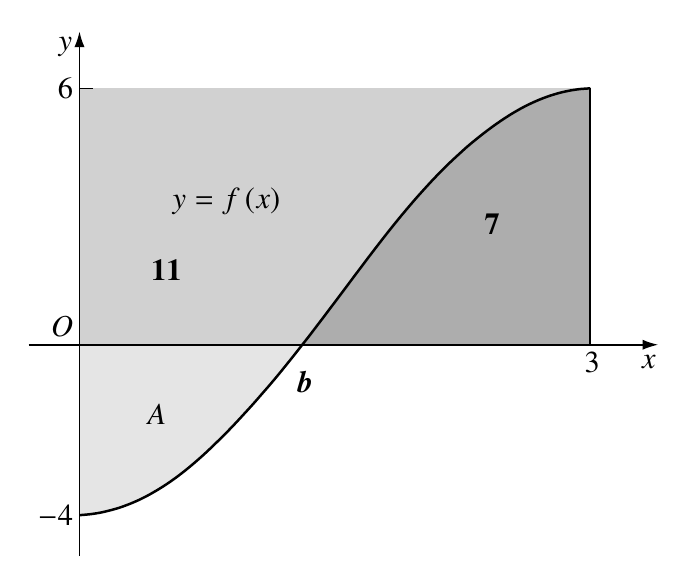
\begin{tikzpicture}[x=0.0127cm,y=-0.0127cm,font=\fontsize{11}{13}\selectfont]
  \fill[black!18] (56,77) rectangle (567,333.5);
  \fill[black!10] plot[smooth] coordinates {(56.0,504.0) (81.0,501.0) (105.0,493.0) (129.0,482.0) (153.0,466.0) (177.0,447.0) (201.0,424.0) (225.0,398.0) (249.0,370.0) (273.0,340.0) (278.0,333.5)} -- (56,333.5) -- cycle;
  \fill[black!32] plot[smooth] coordinates {(278,333.5) (282.4,328.1) (286.8,322.7) (291.1,317.3) (295.5,311.8) (299.8,306.4) (304.1,300.8) (308.4,295.2) (312.7,289.6) (316.9,284.1) (321.2,278.4) (325.4,272.8) (329.7,267.1) (334,261.4) (338.3,255.8) (342.6,250.1) (346.8,244.5) (351.1,239) (355.4,233.4) (359.7,227.9) (364,222.4) (368.3,216.9) (372.7,211.4) (377.1,206) (381.5,200.7) (385.9,195.4) (390.4,190.1) (394.9,184.9) (399.5,179.7) (404.1,174.6) (408.7,169.6) (413.4,164.6) (418.1,159.8) (422.9,154.9) (427.7,150.1) (432.6,145.4) (437.6,140.8) (442.6,136.3) (447.7,131.8) (452.8,127.5) (457.9,123.3) (463.1,119.3) (468.4,115.3) (473.7,111.5) (479.1,107.8) (484.6,104.3) (490.1,101) (495.7,97.87) (501.4,94.91) (507,92.19) (512.9,89.61) (518.7,87.27) (524.5,85.18) (530.5,83.27) (536.4,81.63) (542.5,80.2) (548.5,79.04) (554.6,78.12) (560.8,77.43) (567,77)} -- (567,333.5) -- cycle;
  \draw[->] (5,333.5) -- (635,333.5);
  \draw[->] (56,545) -- (56,20);
  \draw (56,77) -- (70,77);
  \node[anchor=north,inner sep=0pt] at (569,340) {$3$};
  \node[anchor=base] at (625,357) {$x$};
  \node[anchor=base] at (42,39) {$y$};
  \node[anchor=east,inner sep=2pt] at (56,77) {$6$};
  \node[anchor=east,inner sep=2pt] at (56,504) {$-4$};
  \node[anchor=base east,inner sep=2pt] at (56,325) {$O$};
  \draw[line width=0.9pt] plot[smooth] coordinates {(56,504) (66.1,503.1) (76.11,501.6) (86.2,499.3) (96.01,496.5) (105.6,493) (115.2,488.9) (124.7,484.1) (134.1,478.7) (143.3,472.9) (152.4,466.5) (161.4,459.6) (170.1,452.4) (179,444.6) (187.6,436.6) (196.1,428.3) (204.8,419.6) (213.2,410.8) (221.5,401.8) (229.8,392.7) (237.9,383.4) (246,374.1) (254,364.6) (261.9,354.9) (269.7,345.2) (277.4,335.4) (285.2,325.5) (292.9,315.4) (300.6,305.3) (308.2,295.2) (315.9,285) (323.6,274.7) (331.3,264.4) (338.9,254.3) (346.6,244.1) (354.2,234.2) (361.8,224.4) (369.6,214.6) (377.4,205) (385.3,195.6) (393.3,186.3) (401.3,177.4) (409.4,168.6) (417.8,159.9) (426.3,151.5) (434.9,143.5) (443.6,135.6) (452.5,128.2) (461.6,121) (470.9,114.1) (480.2,107.7) (489.5,101.8) (499,96.4) (508.6,91.62) (518.1,87.51) (527.7,84.05) (537.5,81.2) (547.3,79.09) (557.1,77.69) (567,77)};
  \draw (567,77) -- (567,333.5);
  \node at (203,190) {$y=f\,(x)$};
  \node at (133,403) {$A$};
  \node at (143,259) {\bfseries 11};
  \node at (469,213) {\bfseries 7};
  \node at (281,371) {$\boldsymbol{b}$};
\end{tikzpicture}
\end{document}
